\documentclass[]{report}
\usepackage{graphicx}
\usepackage{float}
\usepackage{hyperref}

\begin{document}
	
	\begin{titlepage}
		\centering
		\vspace*{5cm}
		
\includegraphics[width=10cm]{BM.png}
		\vspace*{1cm}
		{\Huge \\ Project Risk Register}
	\end{titlepage}
	
	\section*{Risk Matrix and Usage}
		\begin{figure}[H]
		\centering
		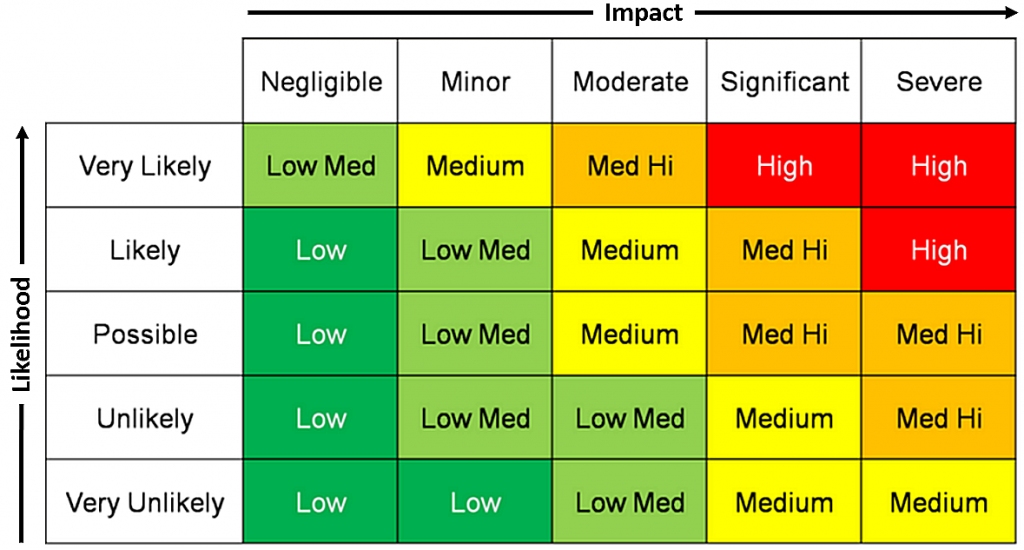
\includegraphics[width=\textwidth]{RiskMatrix.png}
		\caption{Risk Matrix \cite{boers_arms_nodate}}
		\label{fig:risk_matrix}
	\end{figure}
	
	The risk matrix shown in Figure \ref{fig:risk_matrix} will be used to classify each risk that could arise during the development of the project. The categories range between 'Low', 'Medium', and 'High', with 'Low' requiring the least amount of mitigation, and 'High' requiring careful planning to make sure the risk does not become realised.

	\section*{Risk Classification}
	Risks will be described by the following features: \textbf{1.} Description \textbf{2.} Likelihood \textbf{3.} Impact \textbf{4.} Severity \textbf{5.} Role \textbf{6.} Mitigation
	
	\subsection*{Scope Creep}
	\begin{enumerate}
		\item Features of the product becoming more complex without the additional time cost being considered. Leads to the work input to the project being much greater than expected.
		\item Possible
		\item Significant
		\item Med Hi
		\item Project Lead/Technical Lead
		\item List of prioritised features that are highlighted each meeting. Clearly defined goals and a comprehensive success criteria.
	\end{enumerate}
	\subsection*{Unconstructive Communication}
	\begin{enumerate}
		\item Communication relating to the project that does not serve a distinct purpose. Can get stuck in loops of talking about the project instead of solutions within the project as well as including people that do not require as much depth in all communications.
		\item Likely
		\item Minor
		\item Low Med
		\item Project Lead
		\item Create a focused plan for each meeting to ensure key points are discussed. Encourage communication on a need to know basis, clarifying the depth in which each role should be aware of the feature
	\end{enumerate}
	\subsection*{Poor Resource Allocation}
	\begin{enumerate}
		\item Inaccurately estimating the complexity of a task, which can lead to too many or too few personnel working at one time.
		\item Unlikely
		\item Moderate
		\item Low Med
		\item Project Lead
		\item Assign appropriate story points to each task so the real complexity is understood. Dynamically monitor the progress of the task and adjust the allocation in stand-up meetings as needed.
	\end{enumerate}
	\subsection*{Implementation Misunderstanding}
	\begin{enumerate}
		\item Personnel assigned to a task not fully grasping the overall design of the feature, creating discrepancy in the interface being programmed to.
		\item Unlikely
		\item Moderate
		\item Low Med
		\item Technical Lead
		\item Clear communication within the technical team regarding the design of the feature. Check ups when approving each pull request to ensure the design is followed.
	\end{enumerate}
	\subsection*{Unrealistic Timelines}
	\begin{enumerate}
		\item Inaccurately estimating the complexity of a task, which can lead to 'simple' tasks dragging on.
		\item Possible 
		\item Significant
		\item Med Hi
		\item Documentation and Comms
		\item Strong deadlines for functionality combined with the expected complexity that are dynamically adjusted in stand up meetings based on progress.
	\end{enumerate}
	\subsection*{Data Security}
	\begin{enumerate}
		\item Security inaccuracies that can allow private and sensitive data to be revealed without knowledge or permission.
		\item Very Unlikely
		\item Severe
		\item Medium
		\item Data Lead
		\item Responsible storage of project API keys and strictly no sharing. Encryption/hashing on consumer data to ensure no leakage to a third party
	\end{enumerate}
	\bibliographystyle{ACM-Reference-Format}
	\bibliography{rref/rref}
\end{document}